\subsubsection{Konfiguratormenü}

    \begin{figure}[H]
        \centering
        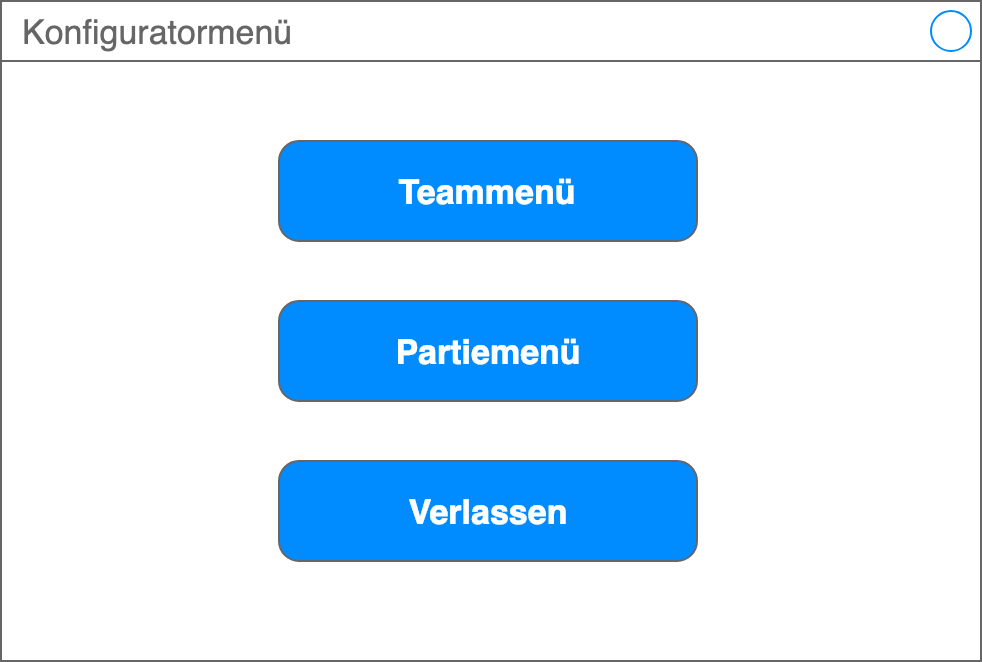
\includegraphics[width=\textwidth/2]{images/konfiguratormenue}
    \end{figure}

    Über das Konfiguratormenü kann eine Auswahl zwischen dem Teammenü und dem Partiemenü über die entsprechenden Buttons getroffen werden. Diese führen zu den Menüs der jeweiligen Konfiguratoren. Über den Button \textit{Verlassen} kann der Konfigurator verlassen werden.

    \subsubsection{Teammenü}
    \begin{figure}[H]
        \centering
        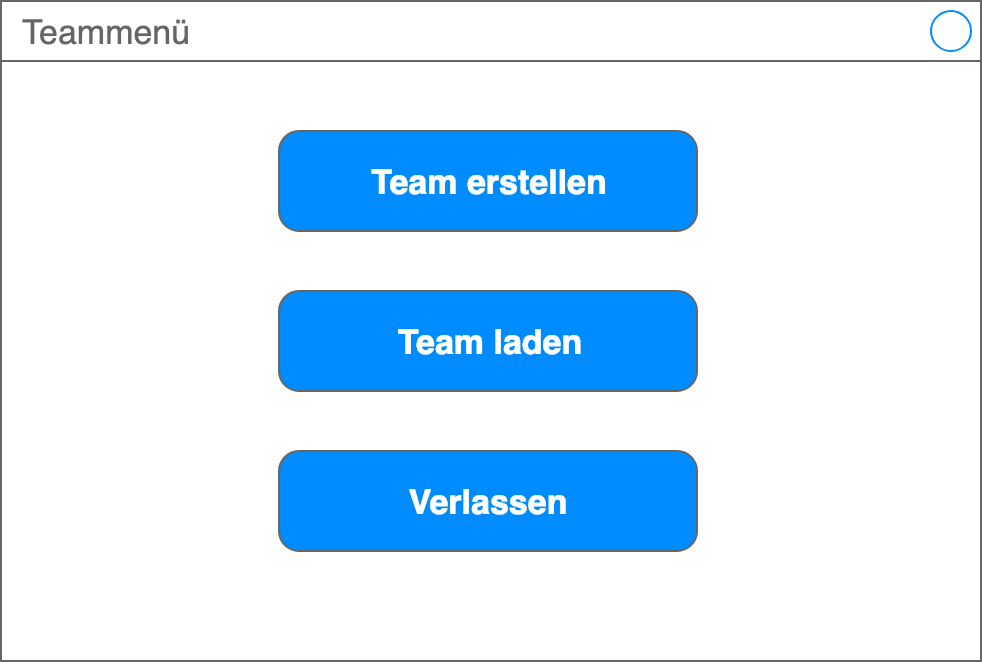
\includegraphics[width=\textwidth/2]{images/teammenue}
    \end{figure}

    Über das Teammenü kann eine Auswahl zwischen dem Laden und dem Erstellen einer Teamkonfiguration getroffen werden. Das erfolgt über die entsprechenden Buttons. Über den Button \textit{Verlassen} kann das Teammenü verlassen werden.

    \subsubsection{Team bzw. Partiekonfiguration laden}

    \begin{figure}[H]
        \centering
        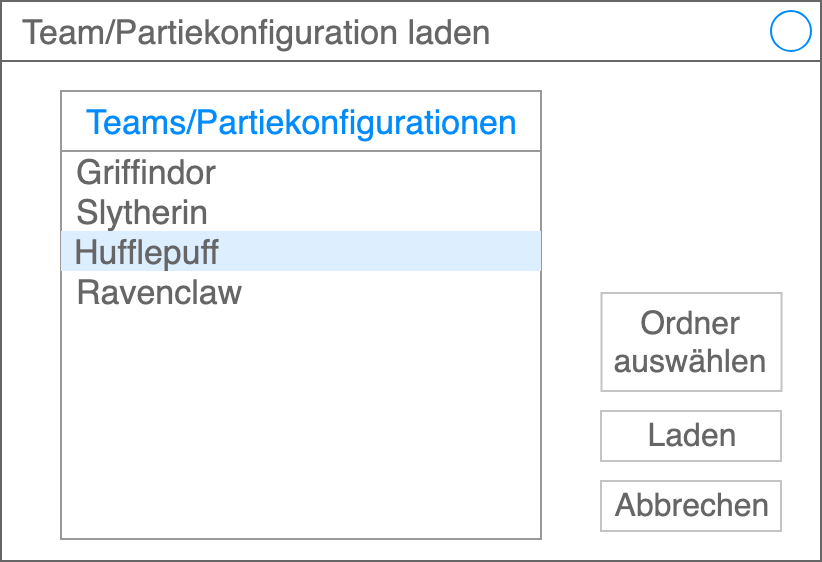
\includegraphics[width=\textwidth/2]{images/laden}
    \end{figure}

    Über diesen Dialog kann eine bereits vorhanden Konfigurationsdatei ausgewählt und im Konfigurator geladen werden. Das erfolgt über ein Dateiauswahlelement und die entsprechenden Buttons. Über den Button \textit{Abbrechen} gelangt man zurück zu den entsprechenden Menüs. Da das Laden einer Teamkonfiguration nahezu identisch zum Laden einer Partiekonfiguration ist, wurde diese beiden Fälle in einem zusammen gefasst. Sollte eine zu ladende Konfigurationsdatei ungültig sein, öffnet sich das Popup \textit{Konfiguration ungültig}.


    \subsubsection{Teamkonfigurator}

    \begin{figure}[H]
        \centering
        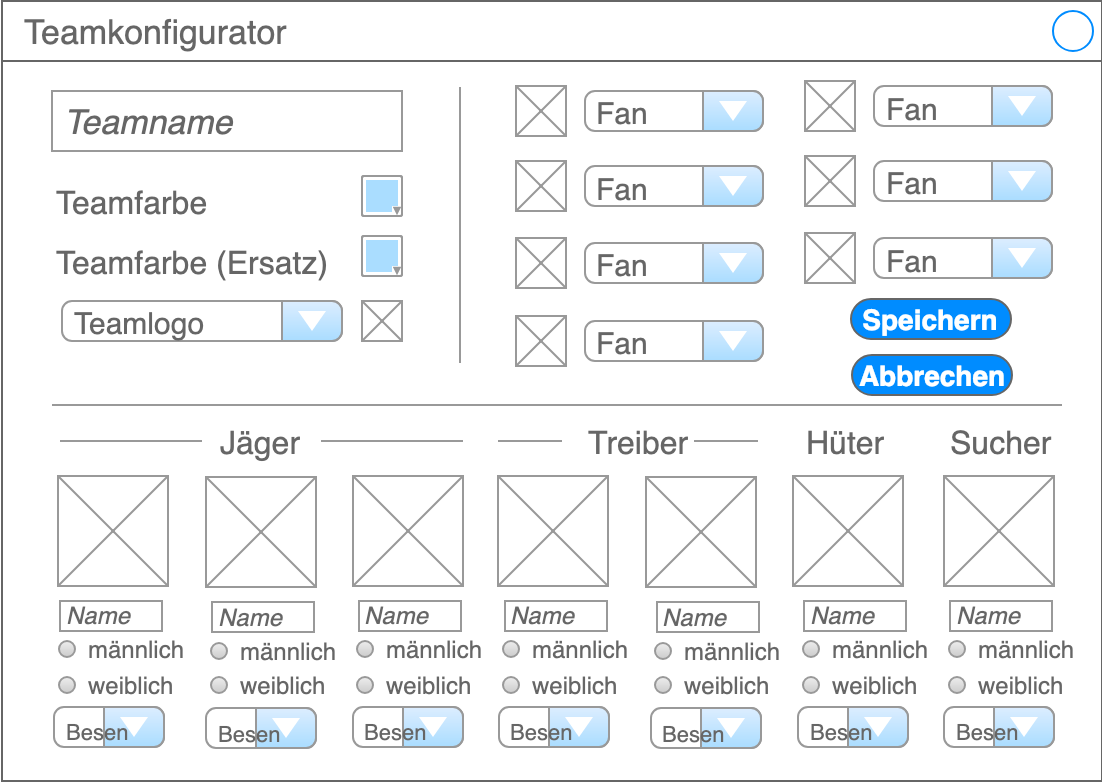
\includegraphics[width=\textwidth]{images/teamkonfigurator}
    \end{figure}

    Im Teamkonfigurator können alle Parameter eines Teams eingestellt werden. Team- und Spielernamen lassen sich durch ein Textfeld bearbeiten. Teamfarben sind über eine Farbauswahl einstellbar. Das Teamlogo lässt sich aus einer Liste vorhandener Logos auswählen. Die Kästen mit den Kreuzen dienen als Platzhalter für Icons, die die verschiedenen Fans und Spieler darstellen und somit unterscheidbar machen. Fans sowie Besen der Spieler sind über eine Dropdown-Auswahl einstellbar. Das Geschlecht der Spieler lässt sich über Radio-Buttons einstellen. Bei jeder Änderung werden die entsprechenden Bedingungen für eine gültige Konfiguration geprüft und der Nutzer erhält visuelles Feedback (z. B. in Form von roter Schriftfarbe in den entsprechenden Feldern). Über den Button \textit{Abbrechen} lässt sich der Konfigurator jederzeit verlassen. Ist eine gültige Auswahl eingestellt, kann die Konfiguration über \textit{Speichern} in einem separaten Speicherdialog persistiert werden.

    \subsubsection{Team bzw. Partiekonfiguration speichern}

    \begin{figure}[H]
        \centering
        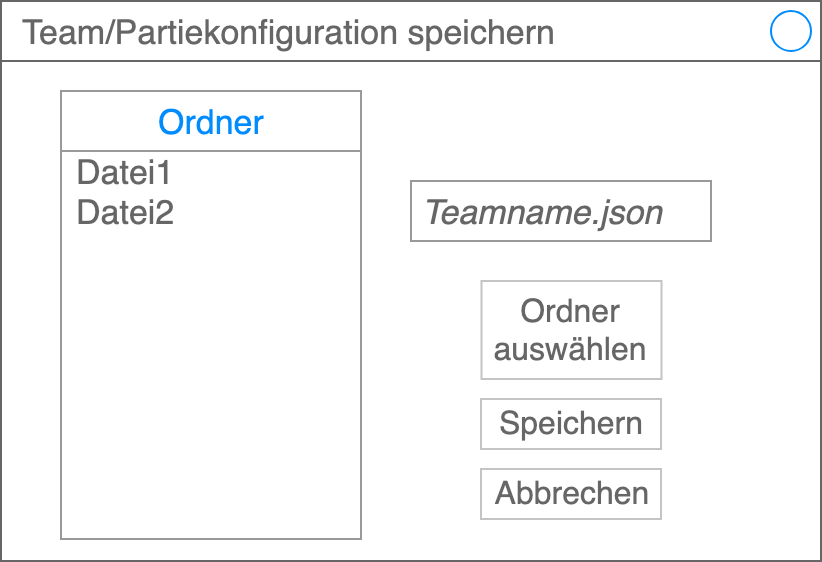
\includegraphics[width=\textwidth/2]{images/speichern}
    \end{figure}

    In diesem Dialog kann Dateiname und Speicherort der Konfiguration festgelegt werden. Der Button \textit{Abbrechen} bringt den Nutzer direkt zurück in den entsprechen Konfigurator. Durch Klicken auf den Button \textit{Speichern} wird die Datei mit dem gewählten Namen und Speicherort gespeichert.

    Wurde versucht eine Konfiguration mit ungültigen Parametern zu speichern oder trat beim Speichervorgang ein Fehler auf, wird der Nutzer über dieses Popup darüber informiert. Der \textit{Ok}-Button führt zurück zum entsprechenden Konfigurator.

    \subsubsection{Konfiguration erfolgreich}

    \begin{figure}[H]
        \centering
        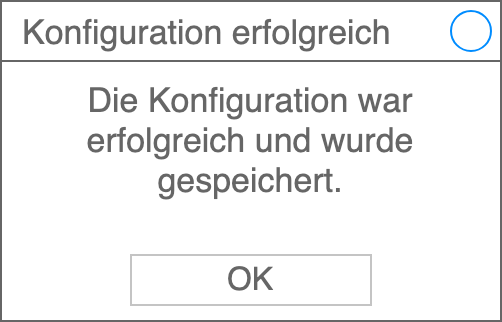
\includegraphics[width=\textwidth/2]{images/konfiguration_erfolgreich}
    \end{figure}

    Wenn alle Paramter einer Konfiguration gültig waren, wird dieser Dialog angezeigt. Der \textit{Ok}-Button führt zurück zum entsprechenden Menü.

    \subsubsection{Konfiguration ungültig}

    \begin{figure}[H]
        \centering
        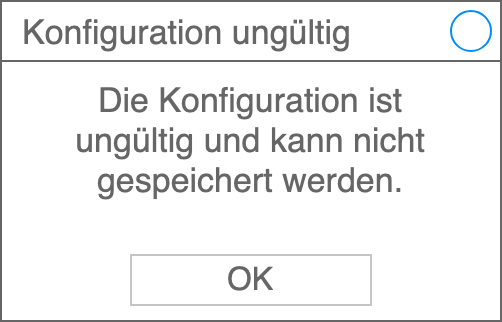
\includegraphics[width=\textwidth/2]{images/konfiguration_ungueltig}
    \end{figure}

    Wurde versucht eine Konfiguration mit ungültigen Parametern zu speichern oder trat beim Speichervorgang ein Fehler auf, wird der Nutzer über dieses Popup darüber informiert. Der \textit{Ok}-Button des Popups führt zurück zum entsprechenden Dialog.

    \subsubsection{Partiemenü}

    \begin{figure}[H]
        \centering
        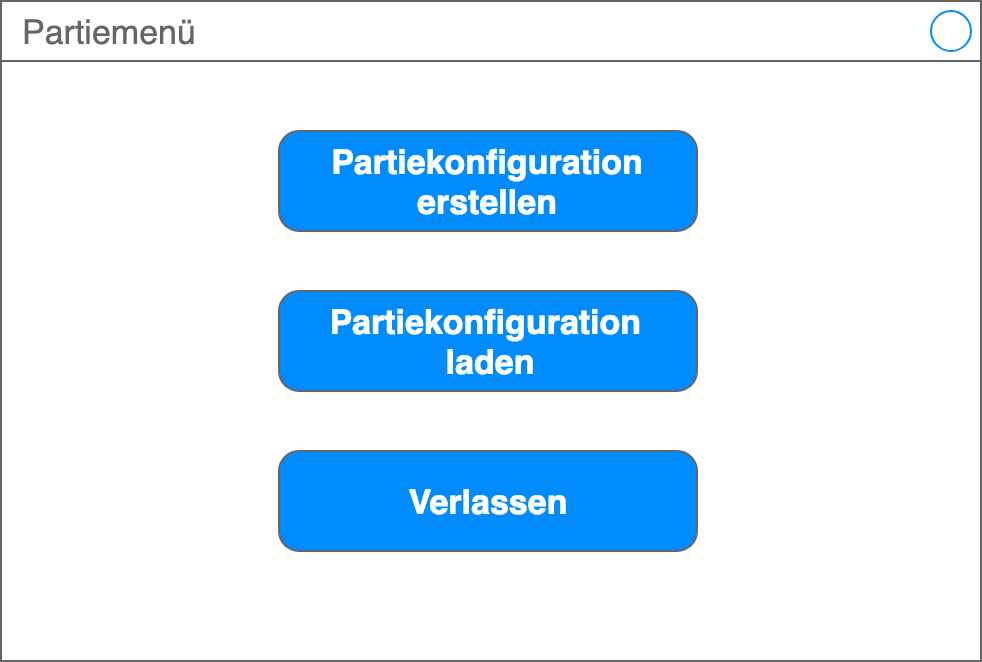
\includegraphics[width=\textwidth/2]{images/partiemenue}
    \end{figure}

    Über das Partiemenü kann eine Auswahl zwischen dem Laden und dem Erstellen einer Partiekonfiguration getroffen werden. Das erfolgt über die entsprechenden Buttons. Über den Button \textit{Verlassen} kann das \textit{Partiemenü} verlassen werden.

    \subsubsection{Partiekonfigurator}

    \begin{figure}[H]
        \centering
        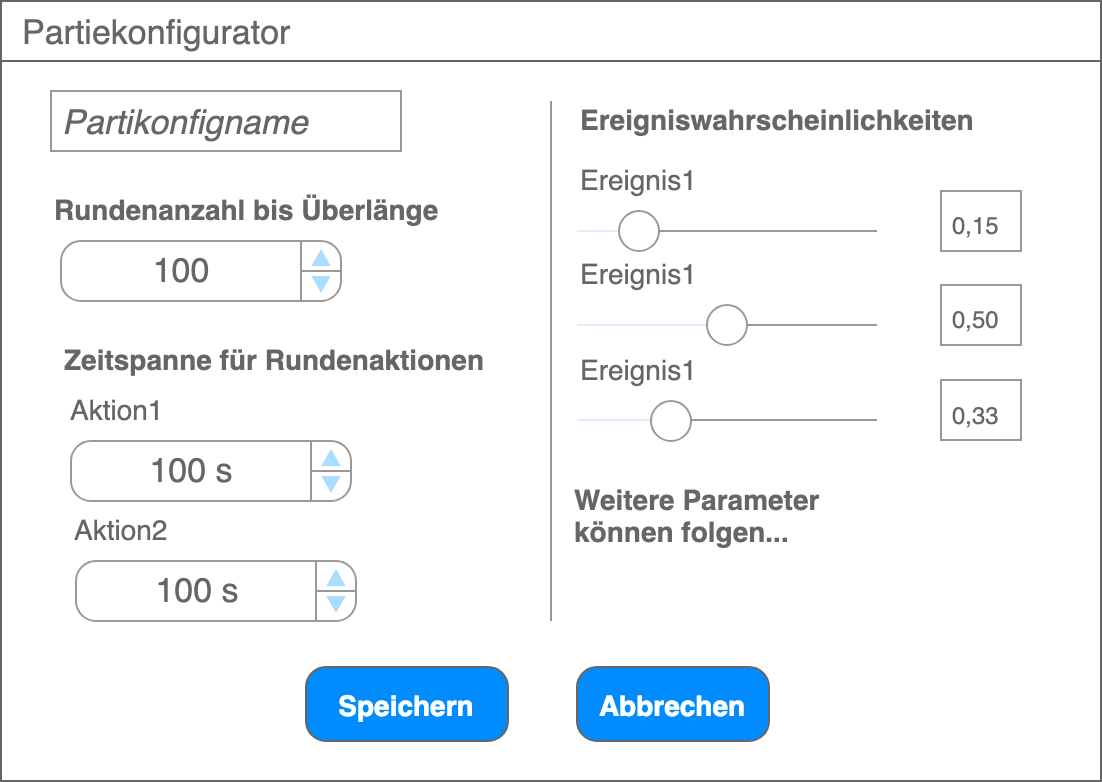
\includegraphics[width=\textwidth]{images/partiekonfigurator}
    \end{figure}

    Im Partiekonfigurator können alle Paramter für eine gültige Partiekonfigurationsdatei eingestellt werden. Dazu gehören unter anderem die Rundenzahl, bis Überlänge erreicht ist, die Zeitspannen für die jeweiligen Spielaktionen und Ereigniswahrscheinlichkeiten. Je nach Art des Parameteres sind Spinner, Slider, Textfelder oder im weiteren Verlauf der Implementierung noch andere Auswahlelemente vorhanden.

    Über den Button \textit{Speichern} gelangt man in den \textit{Partiekonfiguration speichern}-Dialog. Der Button \textit{Abbrechen} führt zurück ins \textit{Partiemenü}.

